\chapter{The Vernier Analysis}
\label{ch:vernier_analysis}
\section{Overview}

The Vernier Scan Analysis is typically done every year, its purpose is to
calculate the absolute luminosity of collisions delivered to PHENIX's
interaction region (IR) by RHIC.  Absolute luminosity is a necessary for the
normalization of any cross-section. This chapter describes the process of
carrying out the vernier analysis for the 2012 data set, but it was also
carried out for the 2013 data set.

A vernier scan describes the process where, one beam is scanned across another
beam held at several fixed positions. The purpose of this maneuver is to enable
direct measurement of the transverse profile of the blue and yellow beam, which
are assumed to be identical. The scanning serves a second purpose, in that, if
one observes the distribution of event collision vertex (in $z$), the shape of
the distribution provides information about the value of the beam focusing
parameter $\beta^*$, and the crossing angle $\theta_{xing}$ between the beams.

Measuring the transverse beam profile allows one to calculate from first
principals the expected machine luminosity delivered to PHENIX,
$\mathcal{L}_{RHIC}$. This luminosity is corrected for both the beam focusing
effect, and the crossing angle. Neglecting to correct both effects will result
in an underestimated luminosity, sometimes by as much as 20\%.

The vernier scan also provides an opportunity to calculate the efficiency of the
minimum bias BBC novertex trigger, which enables the BBCs to be used as a
luminosity monitor for physics operations. 

For the BBC trigger, we represent the relationship between $\mathcal{L}$
and the cross section observed by the BBC as:

\begin{equation} 
\label{eq:lumi_xsec_simple} 
\mathcal{L}_{BBC} = {R_{BBC}\over\sigma_{BBC}} 
\end{equation}

{\noindent}Where $\mathcal{L}_{BBC}$ is the effective luminosity delivered to a
specific BBC trigger, $R_{BBC}$ is the live event rate of the BBC trigger, and
$\sigma_{BBC}$ is defined as the cumulative cross section of events measured by
this trigger.

{\noindent}The absolute luminosity for a single bunch crossing is calculated:

\begin{equation} 
\label{eq:lumi_one_bunch} 
\mathcal{L} = {f_{bunch}N_{b} N_{y}\over{2\pi\sigma_{x}\sigma_{y}}} 
\end{equation}

Where $\mathcal{L}$ is the absolute luminosity, $f_{bunch}$ is the frequency of
each individual bunch crossing, $N_{b}, N_{y}$ are the bunch populations for the
specific blue and yellow beam bunch, respectively, and $\sigma_{x}, \sigma_{y}$
are the transverse widths of both bunches in the $x$ and $y$ directions (see the
PHENIX coordinate system for more details on the origin of these measurements,
Figure~\ref{fig:phenix_coordinate_system}). We assume identical beam bunch
distributions for the blue and yellow beams~\cite{AN888Datta2010}.

Filled bunches cross once every beam clock tick. Therefore, for $120$ bunch
fills (including filled and empty bunches), and the standard blue beam clock
frequency, $f_{clock}$, of $9.36 MHz$, $f_{bunch} \equiv f_{clock} / 120 = 78
kHz$.

This work builds upon previous Vernier Analyses undertaken at PHENIX:
\cite{AN184Belikov2003}, \cite{an597Bazilevsky2007}, \cite{an688Bennett2008},
\cite{AN888Datta2010}, and \cite{Drees2009}.

Global vernier scan characteristics are summarized in table
~\ref{tab:global_scan_summary}. Each vernier scan is done slightly differently
as a systematic check - beam scan order is varied, beam energy is varied, scan
length and step length is varied, and scanning patterns are varied. These
variations are not expected to produce changes in the final luminosity
calculation.

\begin{sidewaystable}[ht]
\centering
\begin{tabular}{ccccccccc}
\toprule
\textbf{Run}    & \textbf{Fill}   & \textbf{Energy}          & \textbf{Scan}       & \textbf{Scan}    & \textbf{Scan}  & \textbf{Beam}    &                & \textbf{Step}     \\
\textbf{Number} & \textbf{Number} & \textbf{($GeV\sqrt{s}$)} & \textbf{Time (min)} & \textbf{Pattern} & \textbf{Order} & \textbf{Scanned} & \textbf{Steps} & \textbf{Time (s)} \\
\midrule
359711 & 16444 & 200 & 41 & Type 1 & H - V & Blue  & 26 & 57.5 \\
360879 & 16470 & 200 & 41 & Type 1 & H - V & Yellow& 26 & 61.2 \\
362492 & 16514 & 200 & 50 & Type 1 & V - H & Blue  & 26 & 62.3 \\
364636 & 16587 & 510 & 58 & Type 2 & H - V & Yellow& 18 & 21.7 \\
365866 & 16625 & 510 & 53 & Type 1 & H - V & Blue  & 26 & 70.0 \\
366605 & 16655 & 510 & 54 & Type 1 & H - V & Yellow& 26 & 67.7 \\
367138 & 16671 & 510 & 54 & Type 1 & H - V & Blue  & 26 & 68.65\\
\bottomrule
\end{tabular}
\caption{ A summary of vernier scans in run 12. Scans which proceed with the
horizontal scan, followed by the vertical scan are denoted `H - V', with the
reverse order denoted similarly. Scan types are defined in
Figure~\ref{fig:scan_patterns}}
\label{tab:global_scan_summary}
\end{sidewaystable}

Two different scanning patterns were used in Run 12, summarized in
Figure~\ref{fig:scan_patterns}. Scan Type 2 was previously used in past years
prior to 2012, and is included in this year's set of scans as a consistency
check. Type 2 scanning describes the pattern where beams begin maximally
overlapped, and are gradually displaced to maximum displacement, brought into
maximum overlap again, then gradually displaced in the opposite direction.  Type
1 was used for the majority of the scans in 2012, and consists of beams
beginning maximally overlapped, subsequently maximally displaced, and swept back
through maximum overlap, continuing, and ending maximally displaced. The scan
order does not effect the final luminosity, provided that beam losses over time
are properly accounted for.

\begin{figure}[ht] 
  \centering
  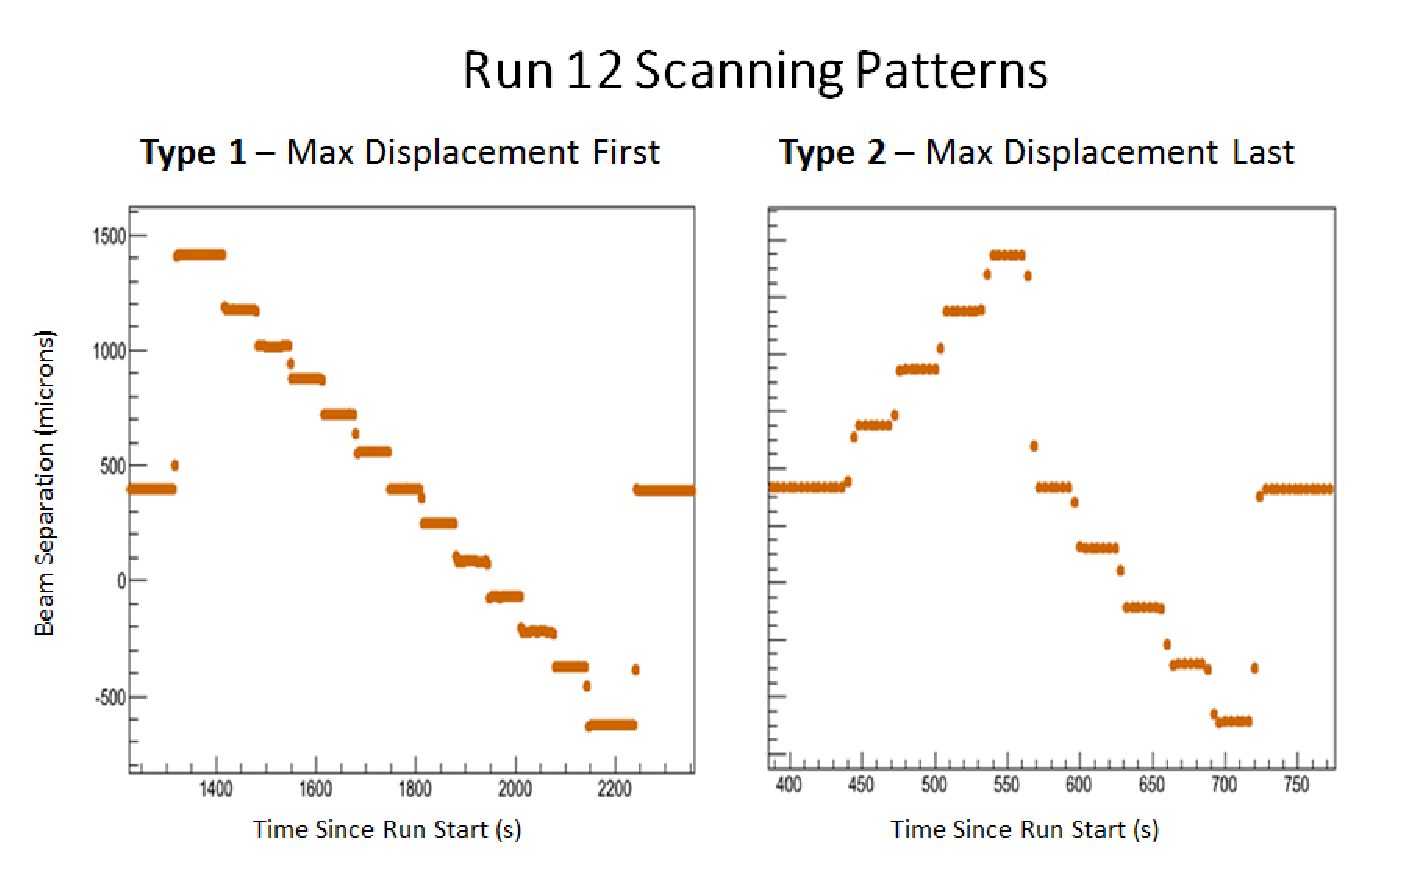
\includegraphics[width=0.75\linewidth]{./figures/scan_patterns} 
  \caption{ 
    Left Panel: Type 1 scanning pattern. Right Panel: Type 2 scanning pattern.
    In both panels, we see the mean beam displacement as a function of time
    since the beginning of the vernier scan.
  }
  \label{fig:scan_patterns}
\end{figure}

\section{Variables and Calculations}
\label{sec:VariablesAndCalculations}

Variables used in the Vernier Analysis are chosen because they characterize the
dynamics of the beams intersecting in the PHENIX interaction region (IR). The
goal in the vernier analysis is to calculate the effective detector cross
section for our Beam Beam Counter, as well as the RHIC machine luminosity,
$\mathcal{L}_{RHIC}$. We must also use a realistic model for highly relativistic
collisions between two intersecting beams.

The basic equations, models and variables used in the analysis are summarized
here. I will go into detail discussing the extraction of each parameter within
relevant section.

The effective detector cross section can be expressed as:

\begin{equation}
  \sigma_{BBC} = {{R_{max}\sigma_x\sigma_y}\over{N_y N_b
\epsilon_{BBC}}}\times{K_{\beta^*}K_{\theta_{xing}}}
\end{equation}

{\noindent}with various parameters are defined in Table~\ref{tab:ana_vars}.
\clearpage
We use the standard relativistic intersecting beam model for
colliding bunches~\cite{AN888Datta2010}, which is defined to be:

\begin{equation}
\label{eq:reletivistic_beam_final} 
\mathcal{L} = {{n_{bunch} f_{bunch} N_{B} N_{Y} }\over{ 2 \pi^{2} \sigma_{x}
\sigma_{y}\sigma{z}^2}} \int \int
e^{-\left({{z^{2}}\over{\sigma_{z}^{2}}}+{{c^{2}t^{2}}\over{\sigma_{z}^{2}}}\right)} c dt
\end{equation}

{\noindent}The full summary of the variables either extracted or directly used
in the vernier analysis are presented in Table~\ref{tab:ana_vars}.

\begin{table}[ht]
  \centering
  \begin{tabular}{c p{9cm} c c }
    \toprule
    \textbf{Variable} & \textbf{Description} & \textbf{Units}  \\
    \midrule 
    $\sigma_{x,y,z} $ & bunch profile width obtained from vernier scan beam
    overlap in $x$, $y$, or $z$ directions. & $\mu m$  \\
    $\sigma_{z}$ & bunch profile width in z-direction, i.e. z-beam width. & $\mu
    m$ \\
    $\dot{N}$ & Live event rate for "BBCLL1(\textgreater0 tubes)" trigger & $Hz$
    \\
    $R_{max}$ & Maximum BBC Rate determined from maximum overlap of beams rate
    for "BBCLL1(\textgreater0 tubes)" trigger & $Hz$ \\
    $R_{MC}$ & Multiple collisions rate & $0 < R_{MC} < 1$ \\
    $\mathcal{L}_{RHIC}$ & Absolute luminosity delivered to PHENIX IR from RHIC
    & $cm^{-2}s^{-1}$ \\
    $\sigma_{p+p} $ & Inelastic scattering cross section of proton-proton
    collisions & $cm^{2}$ \\
    $N_{b}^{i},N_{y}^{i}$ & Number of ions in bunch $i$ for the blue ($b$) beam
    or yellow ($y$) beam. & count \\
    $f_{bunch}$ & Frequency of a specific bunch crossing & $Hz$ \\
    $k_{b}$ & Number of bunches filled in one of the beams (assume identical
    beams) & count \\
    $\sigma_{BBC}$ & Cross section of p+p collisions observed by BBC,
    uncorrected for efficiency & $cm^{-2}$ \\
    $\epsilon_{BBC}$ & BBC efficiency & $0 < \epsilon_{BBC} < 1 $ \\
    $n_{bunch}$ & Number of filled bunches in the blue or yellow beam & $0 \leq
    n_{bunch} < 120$ \\
    $\beta^*$ & Beam focusing parameter, which effectively reduces transverse
    beam width as a function of distance from PHENIX IR. & $cm$ \\
    $\theta_{xing}$ & Crossing angle in the X-Z plane of the blue and yellow
    beams at the intersection point in PHENIX & $mrad$ \\
    $K_{\beta^*}$ & Multiplicative correction to luminosity due to beam focusing
    parameters, $\beta^*$ & - \\
    $K_{\theta_{xing}}$ & Multiplicative correction to luminosity due to beam
    crossing angle.  & - \\
    \bottomrule
  \end{tabular}
  \caption{
    The variables we use in the vernier analysis. Some variables are extracted
    directly from the data streams (such as the bbc-rate), while others are
    calculated from distributions of variables (such as the beam-width,
    $\sigma_{x,y}$). 
  }
  \label{tab:ana_vars}
\end{table}

\section{Data Streams}
\label{ch:DataStreams}

PHENIX software and the overall DAQ structure were discussed in
Chapter~\ref{ch:experimental_apparatus}. The vernier analysis is only interested
in understanding the frequency of minimum bias events, one does not do any
physical event reconstruction beyond determining the event $z$-vertex. To
characterize the vernier scan, the following data streams are used:

\begin{itemize}
\item PRDF Data (available on either 1 second intervals, or event-by-event basis)
  \begin{itemize}
  \item GL1P-0: "BBCLL1(\textgreater0 tubes)"
  \item GL1P-1: "CLOCK"
  \item GL1P-2: "ZDCLL1Wide"
  \item GL1P-3: "ZDCLL1Narrow"
  \item event-sequence
  \item ATP number
  \item epoch time stamp
  \item GL1 crossing ID (bunch number)
  \end{itemize}
\item BPM Data (available in four second intervals)
  \begin{itemize}
  \item Sector 7 Blue Beam x position
  \item Sector 7 Blue Beam y position
  \item Sector 7 Yellow Beam x position
  \item Sector 7 Yellow Beam y position
  \item Sector 8 Blue Beam x position
  \item Sector 8 Blue Beam y position
  \item Sector 8 Yellow Beam x position
  \item Sector 8 Yellow Beam y position
  \item epoch time stamp
  \end{itemize}
\item WCM and DCCT Data (avaialble every few seconds)
  \begin{itemize}
  \item WCM population for each bunch
  \item DCCT beam current for blue beam
  \item DCCT beam current for yellow beam
  \item epoch time stamp associated with each field of WCM or DCCT data
  \end{itemize}
\item DST Data
  \begin{itemize}
  \item BbcOut Node
    \begin{itemize}
      \item BBC pmt tubes fired north
      \item BBC pmt tubes fired south
      \item BBC event z-vertex
    \end{itemize}
  \end{itemize}
  \begin{itemize}
  \item ZdcOut Node
    \begin{itemize}
      \item ZDC event z-vertex
    \end{itemize}
  \end{itemize}
  \begin{itemize}
  \item TrigLvl1 Node
    \begin{itemize}
      \item bitmasked triglive
      \item bitmasked trigscaled
      \item bitmasked trigraw
    \end{itemize}
  \end{itemize}  
  \begin{itemize}
  \item SpinDataEventOut Node
    \begin{itemize}
      \item GL1P crossing ID
      \item event-sequence
      \item GL1P-0: "BBCLL1(\textgreater0 tubes)"
      \item GL1P-1: "CLOCK"
      \item GL1P-2: "ZDCLL1Wide"
      \item GL1P-3: "ZDCLL1Narrow"
    \end{itemize}
  \end{itemize}  
\end{itemize}

The vernier analysis is unique among various PHENIX analyses because it requires
that data streams from RHIC machine sources and the PHENIX detector are
synchronized. It is also unique in that the data set itself exhibits obvious
time dependent behavior. This introduces interesting challenges, as PHENIX
software generally does not provide tools to deal with time dependent data, and
synchronization of PHENIX data with other RHIC data streams is infrequently
done. PHENIX and RHIC data streams effectively live in entirely different
software universes (post data production), so there is no guarantee of a common
key which can be used to synchronize the data. 

\section{Beam Position Monitors}
There are two beam position monitors BPM(s) located about 8 meters away from the
PHENIX IR on either side (BPM sector 7, and BPM sector 8). The BPMs may be used
to establish the relative separation of the blue and yellow beams, but are not
good for establishing absolute beam position~\cite{Drees2013}.  

The BPM data obtained contains measurements of beam position over the course of
an entire fill. The start and end run times recorded in the PHENIX run data
base are used to isolate a chunk of BPM data corresponding to the vernier scan
using epoch time. The BPM data set contains the following fields:
\begin{itemize}
\item epoch time
\item blue beam, sector 7 $x$ position
\item blue beam, sector 7 $x$ position
\item blue beam, sector 8 $y$ position
\item blue beam, sector 8 $y$ position
\item yellow beam, sector 7 $x$ position
\item yellow beam, sector 7 $x$ position
\item yellow beam, sector 8 $y$ position
\item yellow beam, sector 8 $y$ position
\end{itemize}

The beam position monitors are coupled capacitively to the beam
pipe(Figure~\ref{fig:bpm_schematic_cartoon}), with pick ups on the left and
right of the pipe, and pickups above and below the pipe. Every four seconds,
data is read out from the BPMs. 

The method of BPM transduction of beam current to transverse beam position is
described in Figure~\ref{fig:bpm_schematic_cartoon}. The beam current, passing
through the BPM,  induces a time dependent voltage proportional to the
derivative of the beam current itself. BPM electronics use a comparator circuit,
and the readings from pickups situated around the beam pipe are used to
determine the $x$ and $y$ beam positions. The absolute measurement of beam
position is subject to offsets stemming from various effects, but the relative
beam displacement is reliable~\cite{KawallFocus2004}

\begin{figure}[ht]
  \begin{center}
    \includegraphics[width=1.0\linewidth]{./figures/bpm_schematic}
    \caption{ 
      BPM electronics use a comparator circuit, and the readings from X{1,2} and
      Y{1,2} to determine the $x$ and $y$ beam positions. 
    }
    \label{fig:bpm_schematic_cartoon}
  \end{center}
\end{figure}

The BPM data stream provides an $x$ and $y$ position, plus an epoch time stamp
associated with the blue and yellow beams, from sector 7 and sector 8 BPMs.
With this data, one can geometrically extrapolate the intersection of the blue
and yellow beams respectively in the PHENIX IR plane, and then calculate the net
separation between the two beams, Figure ~\ref{fig:bpm_ir_xing_cartoon}.  Three
parallel planes are defined, each plane perpendicular to the beam axis.  One
places the planes at Sector 7 BPM location, the PHENIX IR, and Sector 8 BPM
location.  The two BPM planes are equidistant from the PHENIX IR. One can
geometrically solve for the equation for the line, given intersections at the
BPM Sector 7 plane, and the BPM Sector 8 plane, and extrapolate the beams'
intersection with the IR plane. From this intersection, one obtains the net beam
displacement.

\begin{figure}[ht]
\begin{center}
\includegraphics[width=1.0\linewidth]{./figures/bpm_ir_beam_separation}
\caption{
  Shown: the geometric extrapolation of beam displacement at the IR plane.
}
\label{fig:bpm_ir_xing_cartoon}
\end{center}
\end{figure}


An example of the BPM data recorded during a vernier scan is shown in
Figure~\ref{fig:bpm_data_scan_359711.pdf}, which shows the relative horizontal
and vertical displacements of the beam at the PHENIX IR for run 359711.

\begin{figure}[ht]
  \centering
  \includegraphics[width=0.8\linewidth]{./figures/bpm_data_scan_359711.pdf}
  \caption{
    The horizontal scan is shown in green, with the vertical scan shown in
    purple. Note that relative scan displacements are shown in both the
    horizontal and vertical for the horizontal scan and vertical scan. In this
    case, the blue beam was scanned and the yellow beam was held fixed.
  }
\end{figure}

\clearpage
\section{PHENIX Raw Data} 

The PHENIX raw data format (better known as PRDFs) are the form that recorded
data takes immediately after being assembled into events, by the PHENIX DAQ.
PRDF data is archived soon after being generated on the massive robotic tape
file-system. 

The trigger scalers representing the clock, BBC novertex trigger, BBC 30 cm
cut trigger, and ZDCLL1 trigger are extracted from the PRDFFs.

PRDF data is hierarchical. It is first organized by event-type, and then
organized by packet-type.  Every packet has a header, which contains general
information such as what the packet contains, and in what order that packet was
received from the DAQ. Every packet recorded can be associated with a unique
event-sequence number, which specifies roughly the order in which the event
owning the packet was received by the DAQ. Within a given run number, an
event-number is guaranteed to be unique. The complexity of the packet is limited
by the bandwidth available to move data off PHENIX onto other storage, and the
buffers/reconstruction ability of the front end electronics modules built onto
PHENIX subsystems.

Generally, raw PHENIX data is too complex to use straight-away, because minimal
to no reconstruction of physical properties for a certain event is done (and
this varies by the constraints of each individual subsystem).  However, for the
vernier analysis, we are generally only interested in very simple properties of
an event, all of which are completely available directly from the PRDF. This
allows huge flexibility, as other then the libraries required to dump packet
information from PRDFs headers, there are no dependencies for obtaining the data
we need from PRDFs.

One constraint of using PRDFs as a primary data source is disk space. A normal
physics run may be segmented into hundreds of PRDFs, each at 20 GB in size.
However, because the event rates are on average quite low for a vernier scan,
and because vernier scans typically do not last longer than 20 minutes, there
are typically only five or six PRDFs needed to store an entire scan. The data
extracted from PRDFs is summarized in table~\ref{tab:prdf_data_summary}.

\subsection{GL1-1P Scalers, ATP Numberand Event Time Stamps}

With the DAQ was described in Section~\ref{sec:triggering_aquisition}),
relevant discussion of the DAQ with regards to the Vernier Analysis is discussed
here.

Over the course of the archiving process executed by the DAQ, the event is
categorized by event type.  For this analysis, we consider ``DATAEVENT'' event
types and ``SCALEREVENT'' event types. When data is sent to the ATPs, one of the
64 distinct ATPs will receive each event, depending on which ATP is available to
process an event. Each ATP tags the event it received with an ATP number $0 \leq
ATPNUMBER < 64$, corresponding to the ATP which processed the event and given an
epoch time-stamp. If one desires to use this time stamp, network latency must be
corrected for.

Since time is synchronized between the ATPs via the network, there may be some
latency, which causes a time-offset between the ATPs. However, this latency can
be corrected for.  Because of the large volume of data, several thousand events
will arrive for processing simultaneously, so one can simply choose an ATP (I
choose ``0'') and correct all other time offsets of other ATPs relative to this
time, such that a time offset is obtained in order to synchronize all epoch
times to within one second accuracy for the entire data set.

Other data that are extracted from PRDFS (besides ATPNUMBER, EPOCHTIME,
RUNNUMBER, and EVENTNUMBER) are BUNCHNUMBER, and the GL1-1P scalers.

GL1-1P Scalers are unique counters which may be programmed to track any
arbitrary trigger. These counters count the number of "live" triggers for each
programmed triggers which occur between recorded events. Each time an event is
recorded, the counter dumps the number of "in between" triggers to the GL1P
packet. For Run 12, the triggers programmed into the GL1-1P boards were:

\begin{itemize}
\item BOARD-ID: 0, "BBCLL1(\textgreater0 tubes)"
\item BOARD-ID: 1, "CLOCK"
\item BOARD-ID: 2, "ZDCLL1Wide"
\item BOARD-ID: 3, "ZDCLL1Narrow"
\end{itemize}

To obtain a rate for these trigger scalers, we have two options:
\begin{enumerate}
\item Sum all scalers associated with a single EPOCHTIME to get that scaler's
  per second rate
\item Take the ratio of a particular scaler to the "CLOCK" scaler, converting
  to a rate using the clock frequency ($9.36MHz$).
\end{enumerate}

Both options must yield the same results, unless there are DAQ issues related
to live time. Item 2 is the preferred method, since live-time effects are
nullified by taking the ratio of two run scalers with the same live time, and
all DAQ triggers should generally have the same livetime. Other analyses for
Vernier data have suffered when the CLOCK scaler is not included in the GL1-1P
board programming. In this case, option 1 is the only available option, and the
live-time must be corrected using ratios of live to raw events for each scaler.

\begin{table}[ht]
\centering
\begin{tabular}{ p{2cm} p{5.5 cm} p{6cm} }
\toprule
\textbf{Source} & \textbf{Variable} & \textbf{Application} \\
\midrule 
Event Header & EPOCHTIME & Time ordering data, Calculation of real-time GL1-1P scaler rates \\
 & ATPNUMBER & Synchronization of EPOCHTIME for all events \\
 & RUNNUMBER & Standard PHENIX run ordering  \\
 & EVENTNUMBER & Unique sorting key, proxy for time \\
\midrule
Packet 140008 & GL1-1P 0: ``BBCLL1(\textgreater0 tubes)'' & Counts live events between recorded events \\
              & GL1-1P 1: ``CLOCK'' &  ``'' `` \\
              & GL1-1P 2: ``ZDCLL1Wide''& ``'' ``''\\
              & GL1-1P 3: ``ZDCLL1Narrow''& ``'' ``'' \\
\midrule
Packet 140001 & Gl1-Crossing ID & Identify bunch crossing and used to track beam width, $\sigma_{BBC}$  for specific bunches\\
\bottomrule
\end{tabular}
\caption{ Data extracted from PRDFs. }
\label{tab:prdf_data_summary}
\end{table}

\section{Beam Beam Counter Analysis}

An example of the BBC GL1P scaler for Run 359711 is shown in
Figure~\ref{fig:bbc_gl1p_scaler}, shown alongside the CLOCK GL1P scaler. These
scalers are summed into bins which time order the data. This is accomplished by
ordering the events by the event sequence, which tags events in the order they
were produced. Scalers are summed for every one-thousand events, and then
divided, scaled by the overall CLOCK rate of 9.36 MHz, to produce the BBC event
rate. Note that in the histograms, as the beams are displaced, more and more
clock scalers are recorded, filling the bandwidth, with fewer BBC GL1P scalers.
For maximal overlap, the inverse is true.

\begin{figure}
  \centering
  \includegraphics[width=0.8\linewidth]{./figures/bbc_gl1_scalers.pdf}
  \caption{
    Left: the BBC GL1P scaler plotted as a time series, against an arbitrary
    time proxy. Right: the CLOCK GL1P scaler, plotted in the same way. Both
    distributions are histograms. 
  }
  \label{fig:bbc_gl1_scaler}
\end{figure}

Note that in the event rate, clear divisions appear associated with beam
displacements. When beams are displaced, the event rates drop, but when the
beams are overlapped, the event rates increase. Combining the beam width data
with the rate data is a crucial step in the vernier analysis which allows for
the calculation of the beam width, described in Section~\ref{sec:beam_width}.
The BBC rates for Run 359711 are shown in Figure~\ref{fig:bbc_rate_359711}.

\begin{figure}
  \centering
  \includegraphics[width=0.8\linewidth]{./figures/bbc_rate_359711.pdf}
  \caption{
    Shown: the BBC Rate as a function of time since scan start for Run 359711.
    The stepped distribution is due to changing beam overlap. The rates here are
    intrinsically live-time corrected, because they were generated from the
    ratio of the BBC GL1P scaler and the CLOCK scaler.
  }
  \label{fig:bbc_rate_359711}
\end{figure}

One can estimate the uncertainty associated with the BBC rate by observing the
distribution of the rates around each step. This study is shown qualitatively in
Figure~\ref{fig:bbc_rate_step_dist}, where one can observe histograms for each
scan step of the BBC rate at that particular step. In practice, the average and
RMS is extracted from each distribution.

\begin{figure}
  \centering
  \includegraphics[width=\linewidth]{./figures/359711_bbc_rate_distribution_per_step.pdf}
  \caption{
    In each panel, the BBC rate distribution about a manually defined scan step
    is shown as a histogram. The horizontal is the rate, while the vertical is
    the number of times that a rate bin was observed in the data. From left to
    right, top to bottom, the scan steps are shown, starting at the
    chronologically first step in the top left, and ending with the
    chronologically last step in the bottom right.
  }

\end{figure}

BBC rates may be corrected for multiple collisions per bunch crossing,
Section~\ref{sec:multiple_collisions}. In measurements where overall particle
yield is needed, this correction is vital, however, in our measurement, we care
only about using rates to extract the beam width, as well as calculate the
overall efficiency of the BBC trigger. Other analyses have found that while
rates may change at maximum overlap by as much as 10\%, but was shown to only
affect the beam width by a factor of 1\%.

\clearpage
\subsection{BBC Efficiency}
The efficiency of any detector element can be characterized by addressing the
three following considerations:

\begin{enumerate}
  \item \textbf{Geometric acceptance} (What is the size of the detector? Can particles
    impinging on the detector `miss'?)
  \item \textbf{Physical detector properties} which limit response (i.e. does a
    transducing element operate according to some threshold which may not allow
    it to transduce every particle every time?)
  \item \textbf{Trigger Efficiency}
\end{enumerate}

{\noindent}For the BBCs, items 1 and 3 factor in heavily to its overall
efficiency, $\epsilon_{BBC}$. The ZDC is used to calculate the efficiency of the
BBC. This is possible because the geometric acceptance of the ZDC is relatively
flat with respect to the geometric acceptance of the BBC, concerning particles
which are produced from collisions between the BBCs at $\pm~144cm$.
Schematically, this is shown in Figure~\ref{fig:bbc_geometric_acceptance}. The
geometric acceptance of a detector may be calculated as fraction of the total
solid angle subtended by the detector as seen by an impinging particle from the
event vertex:
\begin{equation}
  BBC_{acc} = {1\over{4\pi}}\left(\int_{\theta_1}^{\theta_2}sin(\theta
    d\theta)\int_{0}^{2\pi}d\phi-\int_{\theta_3}^{\theta_4}sin(\theta)d\theta
    \int_{0}^{2\pi}d\phi\right)
    \label{eq:geometric_acceptance}
\end{equation}

{\noindent}With the first terms in the integral to the left of the `-' sign referring to
the solid angle seen to the left, and the right referring to the solid angle
seen to the right. 

\begin{figure}[hp]
  \centering
  \includegraphics[width=\linewidth]{./figures/geometric_acceptance_noeq.png}
  \caption{
    Shown on the left and right are annular cross-sections of the BBC north and
    south at $\pm~144cm$. The integration bounds in $\theta$
    (Eqtn~\ref{eq:geometric_acceptance}) are labeled, with the distance relative
    to the BBC N and S labeled as $d$, with respect to the event collision vertex
    (the yellow sunburst). Scale is exaggerated to better show the angles.
  }
  \label{fig:bbc_geometric_acceptance}
\end{figure}

One can motivate the use of the ZDC as a calibrating detector for the BBCs with
respect to acceptance by calculating the geometric acceptance of a particle at
all possible event vertices for the BBC and ZDC, and confirming that the
distribution is relatively flat for the ZDC, as seen in
Figure~\ref{fig:solid_angle_compare}.

\begin{figure}
  \centering
  \includegraphics[width=0.8\linewidth]{./figures/solid_angle_compare.png}
  \caption{
    Top: the BBC solid angle as calculated for all possible solid angles within
    the BBC $z$-vertex sensitivity range. Bottom: the solid angle of the ZDC
    seen from an event vertex for all $z$-vertices over the BBC $z$-vertex
    range. Units on the vertical axis are arbitrary for this qualitative
    comparison.
  }
  \label{fig:solid_angle_compare}
\end{figure}

\clearpage
\subsection{Calculation of $\epsilon_{BBC}$}

Analysis in this section focuses on Run 359711, though all scans are analyzed in
a similar manner.

To obtain the BBC efficiency, we must integrate over the BBC trigger acceptance,
while correcting this acceptance for any $z$-vertex dependence. We obtain the
BBC trigger acceptance for the $\pm30cm$ BBC trigger using the BBC trigger with
no vertex cut. First, histograms are generated, observing the yield of particles
associated with various bins of $z$-vertex. We create two such histograms for
the BBC measure trigger acceptance. The trigger acceptance is needed to
determine the effective vertex cut of the BBC $\pm30cm$ trigger, which may not
be precisely $\pm30cm$.

As the baseline, the no vertex cut $z$-vertex distribution is created,
Figure~\ref{fig:bbc_novtxcut}. Then, we fill another histogram only when both
the no-vertex cut and $\pm30cm$ vertex trigger simultaneously fire,
Figure~\ref{fig:bbc_simultaneous}. 

\begin{figure}
  \centering
  \begin{subfigure}[b]{0.7\linewidth}
    \includegraphics[width=\textwidth]{./figures/bbc_wide_zvtx.pdf}
    \caption{BBC wide}
    \label{fig:bbc_novtx_cut}
  \end{subfigure}
  \begin{subfigure}[b]{0.7\linewidth}
    \includegraphics[width=\textwidth]{./figures/bbc_wide_and_narrow_zvtx.pdf}
    \caption{BBC wide and narrow}
    \label{fig:bbc_simultaneous}
  \end{subfigure}
  \caption{
    Panel(a): the $z$-vertex distribution for events that trigger the wide BBC
    trigger. Panel (b): the $z$-vertex distribution for events that trigger the
    BBC wide and narrow triggers.
  }
  \label{fig:acceptance_generators}
\end{figure}

We then create the trigger acceptance plot, bin by bin, dividing the yields per
bin of the no vertex distribution by those of the simultaneously triggered
distribution.  The resulting plot, Figure~\ref{fig:trigger_acceptance} is
produced. From trigger acceptance, one can observe the derivative of the
distribution, to pin point the turn-on position of the online vertex cut. We may
observe the absolute value of the derivative of the trigger acceptance, which
produces two Gaussian peaks centered at the exact locations of the trigger cut
turn on~\ref{fig:acceptance_turn_on}. In this case, for Run 359711, the true
trigger turn on is determined to be events with $z$-vertices between -34.4 cm
and 35.8 cm.

\begin{figure}
  \centering
  \begin{subfigure}[b]{0.7\linewidth}
    \includegraphics[width=\textwidth]{./figures/trigger_acceptance_359711.pdf}
    \caption{Trigger Acceptance}
    \label{fig:trigger_acceptance}
  \end{subfigure}
  \begin{subfigure}[b]{0.7\linewidth}
    \includegraphics[width=\textwidth]{./figures/trigger_acceptance_derivative.pdf}
    \caption{Trigger Turn On}
    \label{fig:acceptance_turn_on}
  \end{subfigure}
  \caption{
    Panel (a) shows the trigger acceptance curve, produced from
    Figure~\ref{fig:acceptance_generators}. Panel (b) shows the absolute
    value of the derivative of (a), with two Gaussian fits to the peak, centered
    at -34.4 cm and 35.8 cm, representing the real trigger turn on.
  }
  \label{fig:acceptance_generators}
\end{figure}

Since $z$-vertex yields may have some $z$-dependence due to geometric acceptance
effects, this must be corrected. To do so, similar distributions of
simultaneously triggered data are generated, however, in this case, we use the
ZDC. In the same vein, the $z$-profile of events triggering the ZDC no vertex
cut is generated, Figure~\ref{fig:zdc_novtxcut}. Additionally, $z$-vertices are
filled into a distribution conditionally, when there is a coincidence of the BBC
no vertex cut trigger and the ZDC no vertex cut trigger
(Figure~\ref{fig:zdc_and_bbc}).

\begin{figure}[hb]
  \centering
  \begin{subfigure}[b]{0.7\linewidth}
    \includegraphics[width=\textwidth]{./figures/zdc_wide_z_359711.pdf}
    \caption{ZDC Wide $z$-vertex}
    \label{fig:zdc_novtxcut}
  \end{subfigure}
  \begin{subfigure}[b]{0.7\linewidth}
    \includegraphics[width=\textwidth]{./figures/zdc_coincidence.pdf}
    \caption{ZDC and BBC coincidence $z$-vertex}
    \label{fig:zdc_and_bbc}
  \end{subfigure}
  \caption{
    Panel (a) shows the wide ZDC $z$-vertex distribution, Panel (b) shows the
    distribution from trigger coincidences between the BBC wide and ZDC wide
    triggers.
  }
  \label{fig:z_dep_generators}
\end{figure}

Finally, a distribution is formed in the same manner as the acceptance
distribution earlier, only this time, this distribution is parameterized with a
fit, Figure~\ref{fig:vertex_correction}. The value of this fit represents the
overall vertex dependence of the BBC no vertex trigger. The correction is
applied as a scaling factor on each $z$-vertex bin of
Figures~\ref{fig:bbc_novtx_cut} and ~\ref{fig:bbc_simultaneous}.

\begin{figure}[ht]
  \centering
  \includegraphics[width=0.8\linewidth]{./figures/vertex_correction.pdf}
  \caption{
    The BBC $z$-vertex correction is obtained from the ratio of BBC and ZDC to
    ZDC yields and fit with a quadratic polynomial. The resulting polynomial is
    used to correct the yields for the BBC coincidence and BBC wide
    distributions, before calculating the total efficiency.
  }
  \label{fig:vertex_correction}
\end{figure}

The final efficiency is calculated by summing the corrected yield of of the
simultaneously triggered BBC yields over the real trigger turn-on interval, and
dividing by the total corrected yield over the full vertex range obtained from
the BBC no vertex distribution. For the case of Run 359711, $\epsilon_{BBC}$ was
calculated to be 0.43.

\clearpage
\section{Wall Current Monitor and Direct-Current Current Transformer}

The wall current monitor (WCM, Figure~\ref{fig:wcm_schematic_cartoon}) and
direct-current current-transformers (DCCT,
Figure~\ref{fig:dcct_schematic_cartoon}) use induced image-charges in plates
capacitively coupled to beam current to measure the total number of ions in the
blue and yellow beams. Additionally, the WCM has timing sensitive enough to
determine individual bunch populations. Since the DCCT is more accurate, it can
be used to calibrate the overall values of bunch populations. The WCMs, because
of their high frequency read out, can even measure the transverse profile of a
single beam-bunch. This profile is necessary for accurate simulation of
collision conditions. Simulations are required to obtain $\beta^*$ and
$\theta_{xing}$ through comparison with the data. This is discussed in
Section~\ref{sec:hourglass_correction}.

Before the WCM data can be used to reckon the population of the beams, they must
be calibrated with the DCCT data. We may calibrate using the following logic: if
the WCM were to provide an accurate measurement of the beam current, then
summing the WCM data over all bunches should yield the same population. However,
since the DCCT is known to be more accurate, we may sum the WCM data, and
normalize to the DCCT. The calibration proceeds as follows:

\begin{gather}
  let~\sum_{i=0}^{N} WCM_{true_{bunch_i}} = DCCT_{total} \\
  then~{{\sum_{i=0}^{N} WCM_{bunch_i}}\over{DCCT_{total}}} = 1 \\
  \therefore WCM_{true} =
  {{DCCT_{total}}\over{\sum_{i=0}^{N}WCM_{bunch_i}}}\times WCM_{bunch_i} \\
  with~WCM_{calib} \equiv {{DCCT_{total}}\over{\sum_{i=0}^{N}WCM_{bunch_i}}}
\end{gather}

{\noindent}With $WCM_{true}$ representing the `correct' value for the WCM by
assuming that the WCM and DCCT must yield the same number for the number of ions
in the beam, a calibration constant is determined for the WCM. The calibration,
$WCM_{calib}$, is applied individually for each matching time index in the time
series data for WCM data and DCCT data.

\begin{figure}[ht]
  \begin{center}
    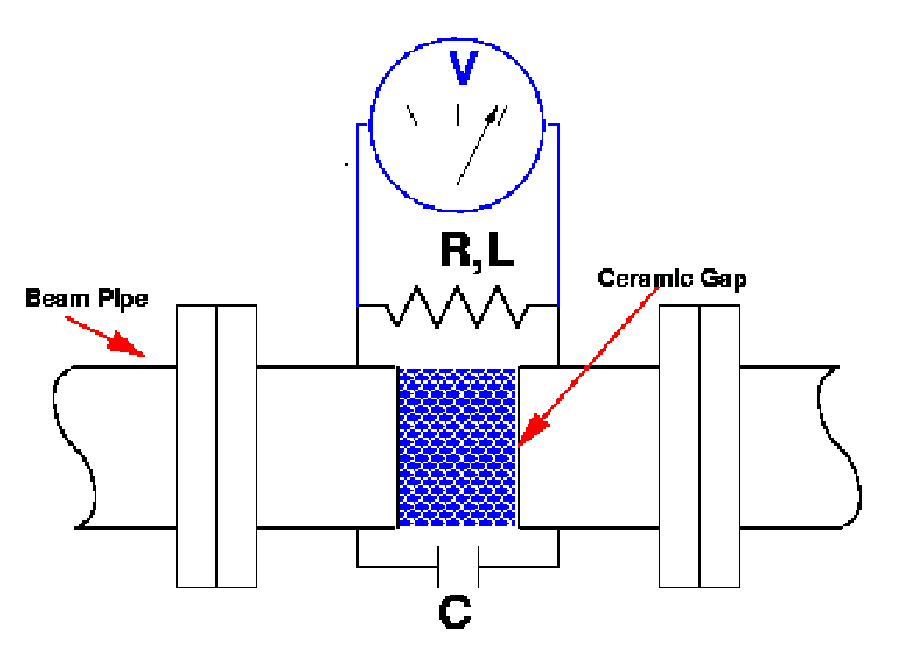
\includegraphics[width=0.75\linewidth]{./figures/wcm_schematic_cartoon}
    \caption{ 
      Shown: an insulating ceramic break in the beam pipe, which shunts
      image wall currents from the beam pipe into the electronics. Magnetic
      shielding excludes external magnetic fields.~\cite{KawallFocus2004} 
    }
    \label{fig:wcm_schematic_cartoon}
  \end{center}
\end{figure}

\begin{figure}[ht]
  \begin{center}
    \includegraphics[width=0.75\linewidth]{./figures/dcct_schematic_cartoon}
    \caption{
      The wall current monitor uses an insulating ceramic break in the beam pipe
      similarly to the DCCT, which forces image wall currents through
      electronics which measure the current frequencies. The WCM is sensitive
      only to bunched beams, and can measure longitudinal profiles of bunches
      ~\cite{KawallFocus2004}.
    }
    \label{fig:dcct_schematic_cartoon}
  \end{center}
\end{figure}

In addition to giving the total beam ion population, as well as the per-bunch
beam ion population, the WCMs also allow us to estimate the rate of beam loss
(Figure~\ref{fig:wcm_rate_loss}), which may impact the overall BBC rate over
time. By taking the product of the blue and yellow beam current, and observing
over the course of a run, one may fit this distribution linearly, and obtain the
per-second percent loss of the beam ion population. Over the course of an entire
vernier scan, this amounts to one percent or less losses, can can be neglected
as a source of rate-loss.

\begin{figure}
  \centering
  \includegraphics[width=\linewidth]{./figures/wcm_rate_loss.pdf}
  \caption{
    Shown: The product of the WCM blue and WCM yellow calibrated data describing
    the total beam ion distribution, as a function of time. This may be used to
    estimate the beam losses due to real ion loss, with the slope representing
    the per-second rate of luminosity loss. In all scans, this amounts to 1\% or
    less for the duration of the scan.
  }
  \label{fig:wcm_rate_loss}
\end{figure}

Finally, we may observe the beam population per bunch using the calibrated WCM
data Figure~\ref{fig:bunch_population_example}. Differences in bunch populations
may be attributed to fluctuation in the way beams are filled, and do not effect
the analyses generally, but should be visualized to determine if there are
drastic fluctuations in beam population which could indicate other problems with
the run.

\begin{figure}
  \centering
  \includegraphics[width=\linewidth]{./figures/359711_bunch_population.png}
  \caption{
    Distribution of WCM population, corrected by DCCT for each bunch for an
    example run. Left: blue beam. Right: yellow beam. For both figures, the
    horizontal axis represents the bunch number.
  }
  \label{fig:bunch_population_example}
\end{figure}

\clearpage
\section{Beam Width Extraction}
\label{sec:beam_width}

\clearpage
\section{Determination of $\beta^*$ and $\theta_{xing}$}
\label{sec:hourglass_correction}

With the addition of a beam focusing parameter, $\beta^*$, and beam crossing
angle, $\theta_{xing}$, the luminosity of intersecting ring particle
accelerators can be boosted by a factor of nearly 20\%. Since the vernier
analysis seeks to calculate the real luminosity, it is important the
characterize the amount that these parameters increase our luminosity. By
observing PHENIX's zero-degree calorimeter's reckoning of the event vertex, at
various beam displacements, one is granted access to observing the effects of
these parameters.

In the model for beam luminosity discussed in Equation ~\ref{eq:lumi_one_bunch},
we neglected to  mention the importance of the $z$-dependent ion distributions
in each bunch. In fact, beam bunches have a $z$-dependent component of their
transverse ion distributions due to the $\beta^*$ beam squeezing. If we could
view the transverse beam width at various points along the bunch in the
$z$-dimension, we would find that the transverse beam width varied as a function
of $z$, Figure ~\ref{fig:beta_squeeze}.

\begin{figure}[h]
  \centering
  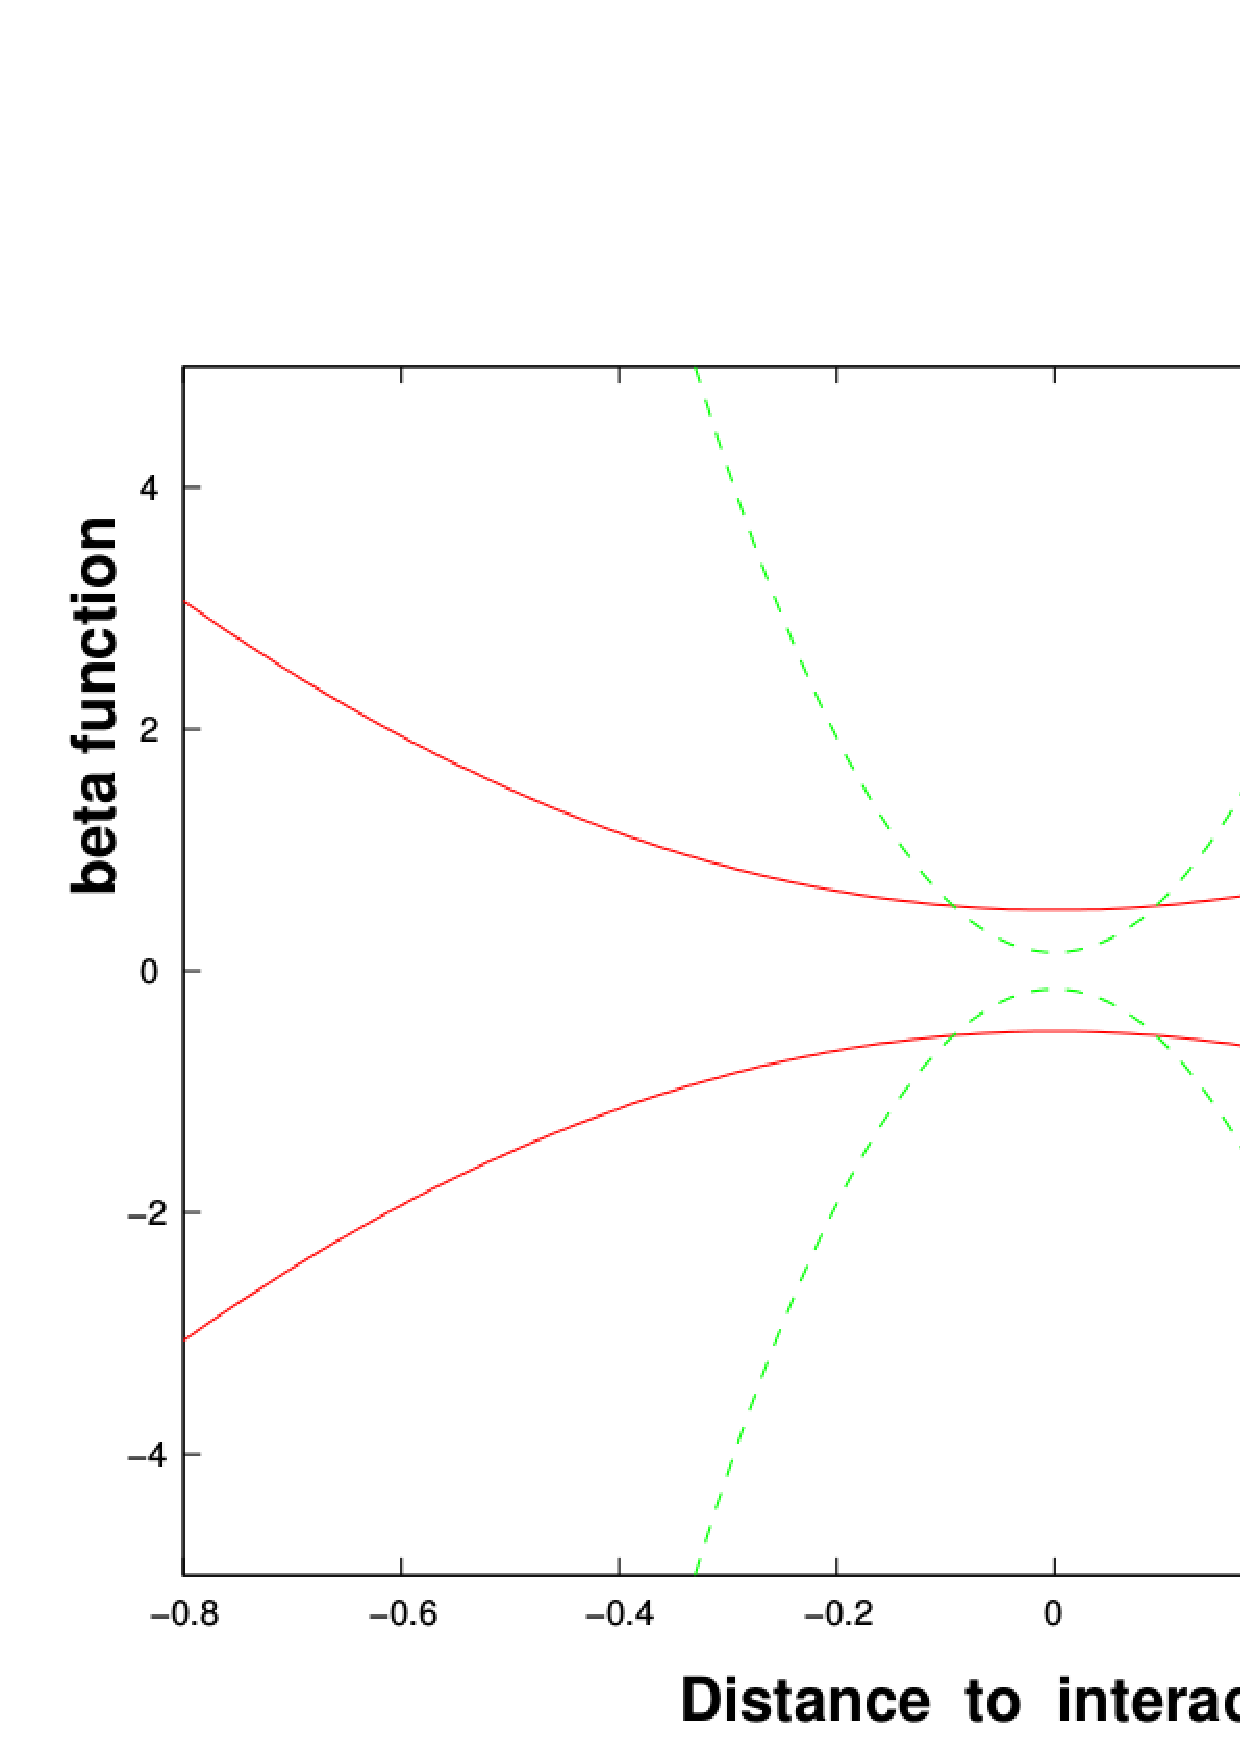
\includegraphics[width=0.8\linewidth]{./figures/beta_function.png}
  \caption{
    A cartoon is shown for various potential values of $\beta^*$, showing the
    squeezing transverse profile~\cite{Herr2003a}.
  }
  \label{fig:beta_squeeze}

\end{figure}

A better model for the beam geometry without defining simple Gaussian geometry
is defined:
\begin{equation}
\label{eq:generalluminosity}
\mathcal{L} = 2N_{blue}N_{yellow}f_{bunch}N_{bunch}\iiiint _{\infty}^{ \infty}{
\rho_{blue} (x,y,z-ct_0)\rho_{yellow} (x,y,z+ct_0)} dxdydzdt
\end{equation}
If the densities in equation~\ref{eq:generalluminosity} are simplely Gaussian,
the normalizations may be extracted from the integrand, and the integration can
be performed analytically. This simple geometry is shown in
Figure~\ref{fig:simple_bunch_xing}.

\begin{figure}
  \centering
  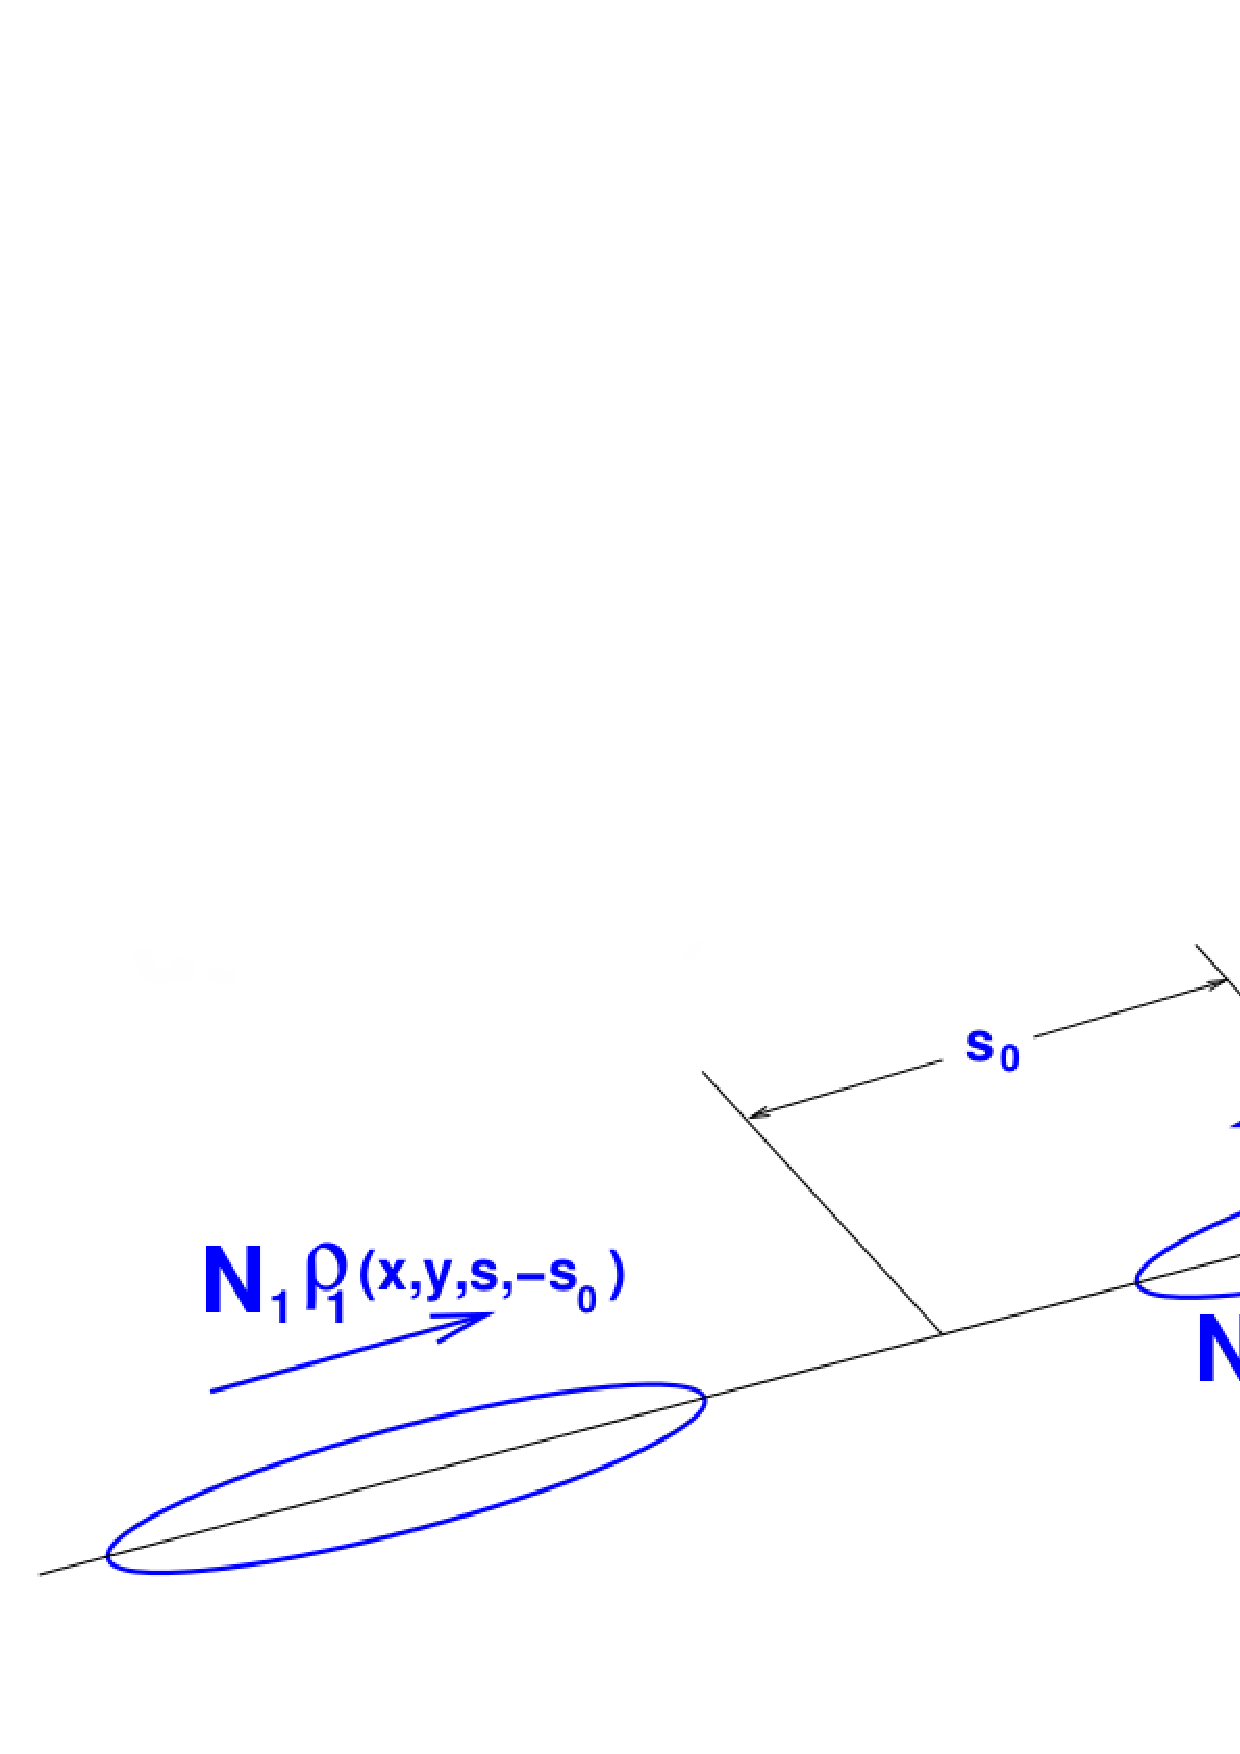
\includegraphics[width=0.75\linewidth]{./figures/simple_bunch_head_on.png}
  \caption{
    Shown: a simple bunch collision with no crossing angle or beam focusing with
    Gaussian bunch profiles in $x$,$y$, and $z$,~\cite{Herr2003a}.
  }
  \label{fig:simple_bunch_xing}
\end{figure}

The simple normalized Gaussian beam profile for any single dimension, $x_i, i=x,
y, z$  may be written, and normalized as follows:

\begin{equation}
\label{eq:simplegaussian}
\rho(x_{i}) = \frac{e^{ -\frac{(x_{i}-\mu)^2}{2\sigma_{x_i}^2}}}{\sigma_{x_i}\sqrt{2\pi}}
\end{equation}

{\noindent}If all profiles are of this form, then the densities are separable,
and we may perform the integration. However, higher order beam effects introduce
complications which will prevent us from separating the densities, as well as
performing the integration analytically.

The beam crossing angle is assumed to occur only in the $x$-$z$ plane. This
assumption is motivated physically, as the RHIC accelerator is positioned such
that the beams circulate in a path constrained to a flat plane. 

One can apply transformations~\ref{fig:bunch_transform} to the basic Gaussian
beam profile to generate the most realistic overlap integral. Once we have a
form that is representative of the real overlap conditions, we may integrate out
the $x$ and $y$ degrees of freedom, leaving a distribution in $z$ and $t$. This
distribution is sampled randomly to create a simulated $z$-vertex profile. These
transformations represent the effects of the crossing angle and the beta-squeeze
at the PHENIX IR.


\begin{figure}[ht]
  \centering
  \begin{subfigure}[b]{\textwidth}
    \centering
    \includegraphics[width=\linewidth]{./figures/bunch_rotation.png}
    \caption{Rotation to coordinates representing crossing angle~\cite{Herr2003a}}
  \end{subfigure}
  \begin{subfigure}[b]{\textwidth}
    \centering
    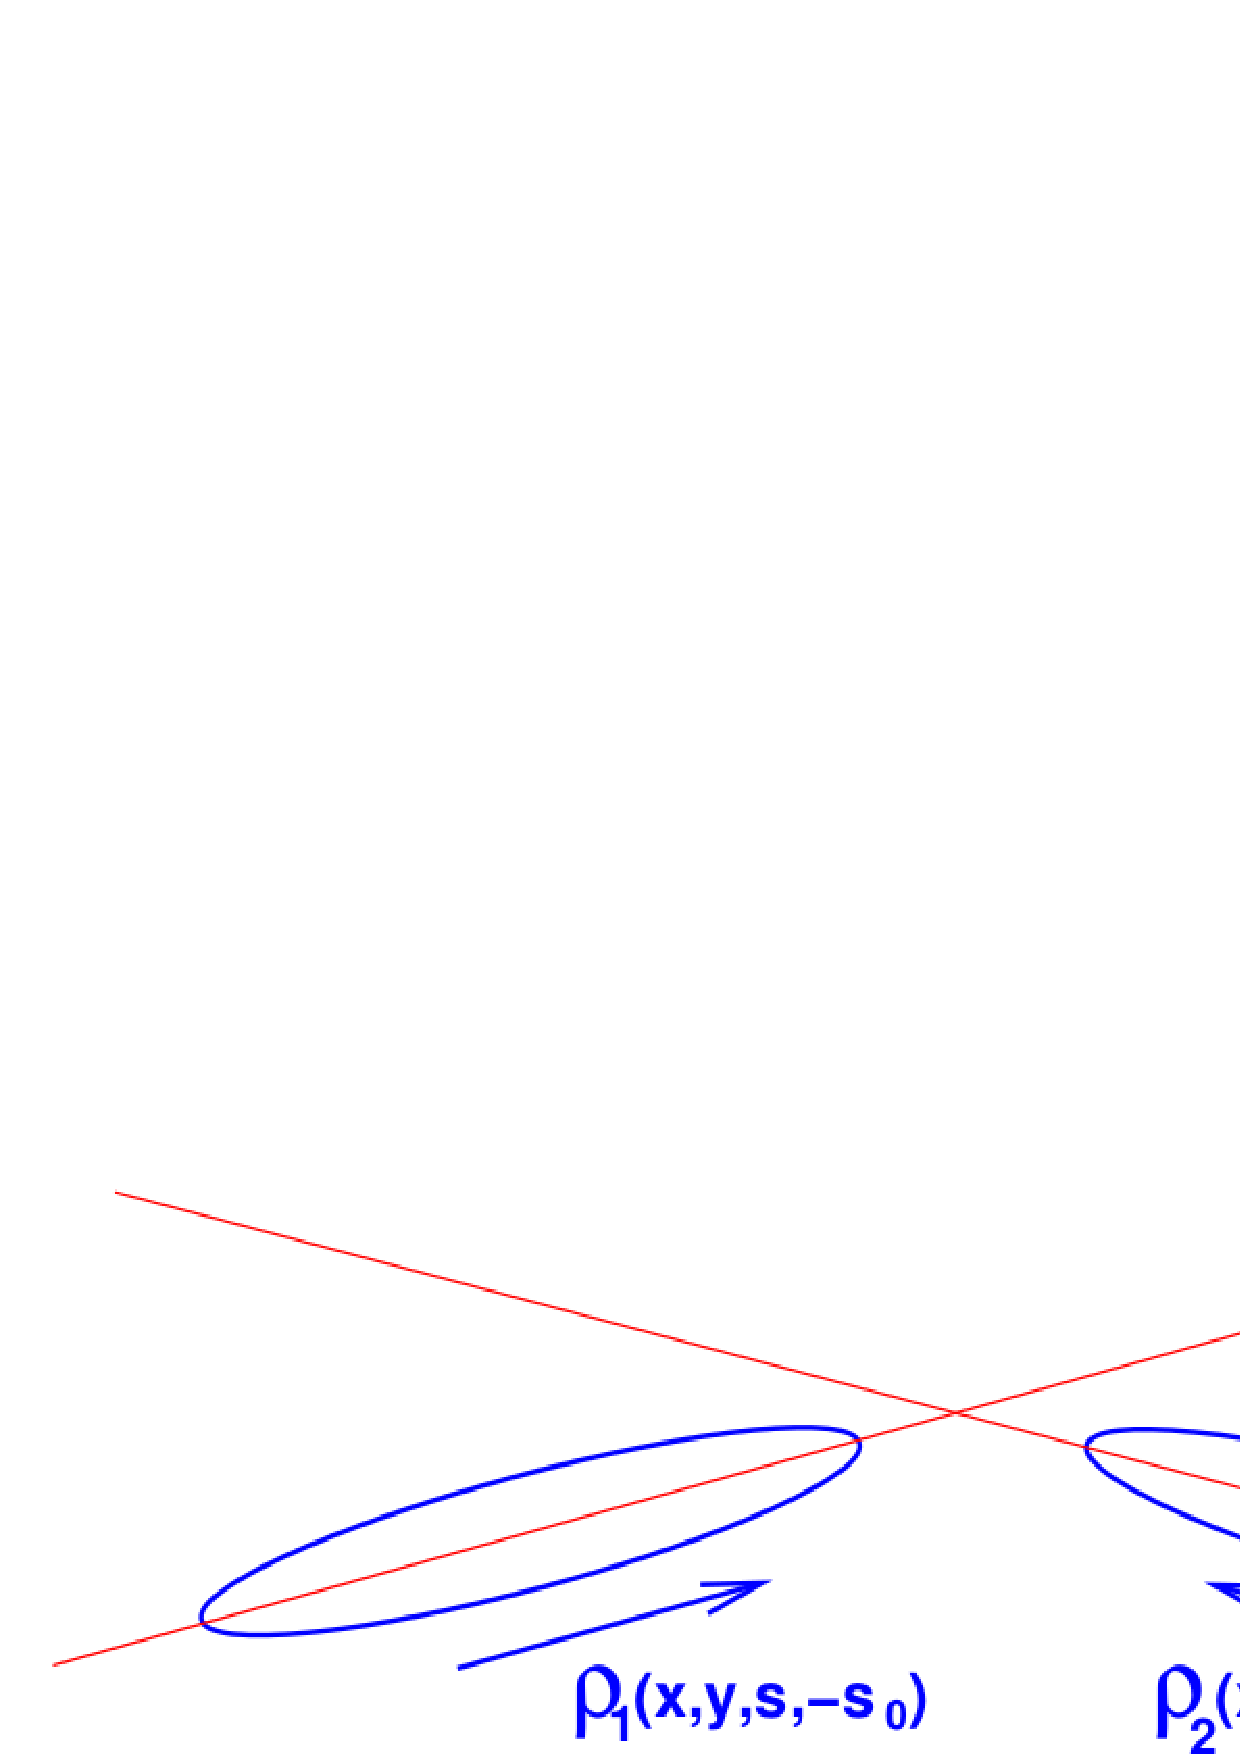
\includegraphics[width=\linewidth]{./figures/xing_bunch.png}
    \caption{Bunches colliding at an angle~\cite{Herr2003a}}
  \end{subfigure}
  \caption{
    Panel (a) shows the coordinate transformation applied to the bunch profiles
    which resulting in a crossing angle, with Panel (b) depicting the result.
  }
  \label{fig:bunch_transform}
\end{figure}
\clearpage
The results of this rotation are described, assuming a small crossing angle,
known to be within $\vert\theta_{xing}\vert < 2~mrad$:

\begin{gather}
\label{eq:transformations}
x_{blue}   \rightarrow x cos \frac{\phi}{2} - z sin \frac{\phi}{2} \\
z_{blue}   \rightarrow z cos \frac{\phi}{2} + x sin \frac{\phi}{2} \\
x_{yellow} \rightarrow x cos \frac{\phi}{2} + z sin \frac{\phi}{2} \\
z_{yellow} \rightarrow z cos \frac{\phi}{2} - z sin \frac{\phi}{2} \\
sin \frac {\phi}{2} \rightarrow \frac{\phi}{2} \\
cos \frac {\phi}{2} \rightarrow 1 + \frac{\phi^2}{4}
\end{gather}

{\noindent} with the beta squeeze transforming the profiles as:

\begin{equation}
\label{eq:beta_star_transform}
\sigma_{x_i} \rightarrow \sigma_{x_i} \sqrt{1+\left(\frac{z}{\beta^*}\right)^2 }
\end{equation}

{\noindent} in the transverse directions.

With proper transformations applied to represent the beta squeeze and crossing
angle, we may proceed with simulation, provided a realistic $z$-profile can be
obtained. Fortunately, the WCM data provides such a profile, and one may fit
this profile, as shown in Figure~\ref{fig:z_profile}.

\begin{figure}
  \centering
  \begin{subfigure}[b]{0.8\textwidth}
    \centering
    \includegraphics[width=\linewidth]{./figures/blue_zprofile_359711.pdf}
    \caption{The blue beam profile}
  \end{subfigure}
  \begin{subfigure}[b]{0.8\textwidth}
    \centering
    \includegraphics[width=\linewidth]{./figures/yell_zprofile_359711.pdf}
    \caption{The yellow beam profile}
  \end{subfigure}
  \caption{
    A parameterization of the blue beam profile in $z$ is shown in Panel (a),
    with the yellow in panel (b). Included are the resulting fits by
    parameterizing the profiles with a triple-Gaussian fit, with parameters 2, 5
    and 8 referencing the widths of the distributions.
  }
  \label{fig:z_profile}
\end{figure}

Under normal collision conditions, we expect a gaussian distribution in the
$z$-vertex profile, as seen in Figure~\ref{fig:zdc_zprofile_max_overlap}. This
makes intuitive sense, if both beam profiles are even moderately
Gaussian-shaped. Collisions are most likely when the densest part of the beam
profile are overlapped, and beams are enginnered to overalp maximally at $z=0$
in the PHENIX coordinate frame.

\begin{figure}[ht]
  \centering
  \includegraphics[width=0.8\linewidth]{./figures/zdc_zvtx_max_overlap_359711.pdf}
  \caption{
    Shown: the ZDC $z$-vertex collision profile for beams colliding at maximum
    overlap. 
  }
  \label{fig:zdc_zprofile_max_overlap}
\end{figure}

As the bunch becomes more diffuse towrads the periphery, collisions may still
occur, as the dense central region of each bunch overlaps with the less diffuse
areas of the other bunch (visualized in Figure~\ref{fig:beam_profile_overlap}).


\begin{figure}[ht]
  \centering
  \begin{subfigure}{0.7\linewidth}
    \includegraphics[width=\textwidth]{./figures/359711_time_step_0_bunch_collision.pdf}
    \caption{Before}
  \end{subfigure}
  \begin{subfigure}{0.7\linewidth}
    \includegraphics[width=\textwidth]{./figures/359711_time_step_1_bunch_collision.pdf}
    \caption{Collision}
  \end{subfigure}
  \begin{subfigure}{0.7\linewidth}
    \includegraphics[width=\textwidth]{./figures/359711_time_step_2_bunch_collision.pdf}
    \caption{After}
  \end{subfigure}
  \caption{
    Shown: a cartoon of realistic beam profiles before (Panel (a)) collision,
    during collision (Panel (b)), and after collision (Panel(c)).
  }
  \label{fig:beam_profile_overlap}
\end{figure}

When beams are not maximally overlapped, one may observe the effects of both the
beta squeeze and the crossing angle, collectively termed the `hourglass effect'.
The term refers to the shape of the zdc $z$-vertex profile associated with
displaced beams, which looks like an hourglass turned on its side. This effect
is most apparent at beam overlap relative to the total transverse beam width.
One sees a double-peak structure, which is due to the $\beta^*$ squeezing
parameter and an asymmetry of peak-height which is due to the crossing angle,
shown in Figure~\ref{fig:zdc_beam_displacement}. 

\begin{figure}[h]
  \centering
  \includegraphics[width=0.8\linewidth]{./figures/zdc_zvertex_max_displacement_359711.pdf}
  \caption{
    Shown: With a large displacement in the beams, the hourglass effect can be
    seen in the ZDC $z$-vertex profile.
  }
  \label{fig:zdc_beam_displacement}
\end{figure}


We cannot recover the parameters to the shape of this distribution with fitting,
but we can simulate the collision conditions, and match the simulation to the
data. To avoid the pitfalls of overtuning the simulation and recovering the
wrong parameters of $\beta^*$ and $\theta_{xing}$, I developed a root-finding
algorithm which performs a binary search over the parameter space of the
simulation (described in Table~\ref{tab:hourglass_simulation_parameters}) with
the Multiple Collisions rate (Section~\ref{sec:multiple_collisions}), the
crossing angle, and the $\beta^*$ parameters allowed to vary over a wide range.  

\begin{table}[h]
  \centering
  \begin{tabular}{c p{10cm}}
    \toprule
    \textbf{Parameter} & \textbf{Description}\\
    \midrule
    $\beta^*$ & Beam focusing parameter which causes offset beams to follow a
    dual-peak structure \\
    $\theta_{xing}$ & The beam crossing angle in the $x$-$z$ plane relative to
    the PHENIX coordinate system. Causes an asymmetry in the observed peaks. \\
    $R_{MC}$ & Multiple collision rate. Causes scaling of the overall
    distribution towards the center, at $z=0$. \\
    $\sigma_{x,y}$ & Transverse beam widths. Along with the beam displacement,
    effects the threshold separation where $\beta^*$ and $\theta_{xing}$
    effects are obviously observed by eye \\
    {X,Y}\_OFFSET & The beam offset in the x and y directions. Along with the
    transverse beam width, these parameters effect the threshold where the
    hourglass effect can be observed by eye. \\
    \bottomrule
  \end{tabular}
  \caption{
    The parameters characterizing the hourglass simulation are described.
    Though the nomralization of the luminosity describing the final $z$-vertex
    profile with a fixed offset depends on many parameters, only parameters shown
    actually effect the shape of the distribution.
  }
  \label{tab:hourglass_simulation_parameters}
\end{table}

Convergence in the simulation is tested by weighting the least-squares
difference between the simulation and data by the uncertainty of the data for
each $z$-vertex bin in the data sample.  When the algorithm executes, a clear
convergence of the least-squares residual is observed
(Figure~\ref{fig:least_squares_convergence}), indicating success.
Schematically, the simulation is diagrammed in Figure~\ref{fig:simulation_flow}.
The algorithm is halted after fifteen iterations, which is typical of the binary
search, since each iteration halves the next step in the search domain and after
fifteen iterations the step size changes are on the order of 1 part in 100,000. 


\begin{figure}[h]
  \centering
  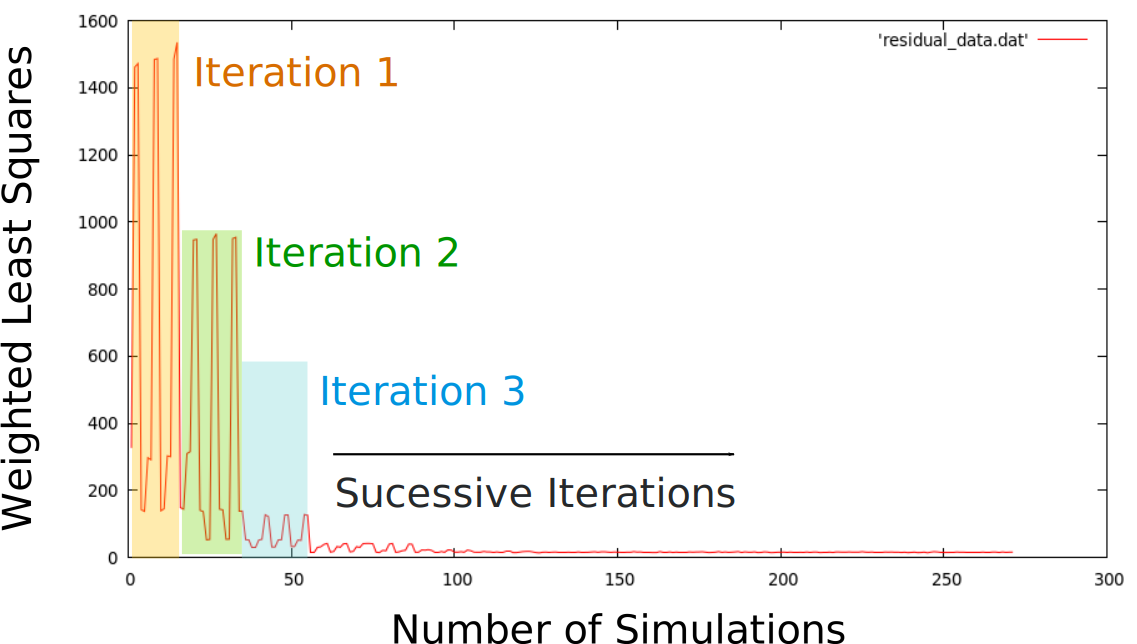
\includegraphics[width=0.8\linewidth]{./figures/vernier_root_finding.png}
  \caption{
    The least-squares residual is shown to be converging with each
    successive iteration of the algorithm. Modulation in the parameter within
    each iteration is a result of the binary search executing and finding the
    best set of parameters to keep for the next iteraiton.
  }
  \label{fig:least_squares_convergence}
\end{figure}


\begin{figure}[h]
  \centering
  \includegraphics[width=0.8\linewidth]{./figures/simulation_flow.pdf}
  \caption{The schematic algorithm for the hourglass simulation.}
  \label{fig:simulation_flow}
\end{figure}

With the binary search algorithm in place, we may now recover the value for
$\beta^*$, $\theta_{xing}$, and $R_{MC}$. Examples of convergent distributions,
along with the final best parameters characterizing the shape of the ZDC
$z$-vertex profile are summarized in Figures~\ref{fig:profile_1} -
\ref{fig:profile_4}. Though many parameters are shown alongside each simulation,
the parameters listed outside of Table~\ref{tab:hourglass_simulation_parameters}
do not effec the overall shape of the distribution, but can be used to calculate
an overall luminosity associated with colliding beams at a fixed offset. Since
the luminosity of interest is only when beams are overlapped maximally, these
parameters are not used, but are kept for potential future cross-checks.

\begin{figure}
  \centering
  \includegraphics[width=\textwidth]{./figures/65_micron_step.pdf}
  \caption{
    Shown: the convergence of the $z$-profile simulation after 15 iterations for
    a $65~\mu m$ beam displacement. 
  }
  \label{fig:profile_1}
\end{figure}

\begin{figure}
  \centering
  \includegraphics[width=\textwidth]{./figures/971_micron_step.pdf}
  \caption{
    Shown: the convergence of the $z$-profile simulation after 15 iterations for
    a $971~\mu m$ beam displacement. 
  }
  \label{fig:profile_2}
\end{figure}

\begin{figure}
  \centering
  \includegraphics[width=\textwidth]{./figures/1105_micron_step.pdf}
  \caption{
    Shown: the convergence of the $z$-profile simulation after 15 iterations for
    a $1105~\mu m$ beam displacement. 
  }
  \label{fig:profile_3}
\end{figure}

\begin{figure}
  \centering
  \includegraphics[width=\textwidth]{./figures/more_statistics.pdf}
  \caption{
    Shown: the convergence of the $z$-profile simulation after 15 iterations for
    a $1004~\mu m$ beam displacement. 
  }
  \label{fig:profile_4}
\end{figure}

With a strategy to recover $\beta^*$ and $\theta_{xing}$, we may proceed with
implimenting the corrections for these effects to the total luminosity. This is
done separately from the simulation, with the full form of the Luminosity being
numerically integrated with all relevant parameters calculated or extracted from
the data streams.

{\noindent}The effect of $\beta^*$ is used to correct total luminosity according to:
\begin{gather}
  L\sim \iiiint \rho_{blue}(x,y,z,t)\dot\rho_{yellow}(x,y,z,y)dxdydzdt \\
  \rho(x,y,z,t) = \rho(x)\rho(y)\rho(z-ct) \\
  \rho(x_i) = {{1}\over{\sigma(z)_{x_i}
  \sqrt{2\pi}}}e^{-\left({{x_i-x_0}\over{2\sigma(z)_{x_i}}}\right)^2}~(x_1 = x, x_2
  = y)\\
  \sigma_{x_i}(z\vert_{z=0})^2\left(1+\left({{z}\over{\beta^*}}\right)^2\right) \\
  K_{\beta^*} =
{{\mathcal{L}_{\beta^*\rightarrow\infty}}\over{\mathcal{L}_{\beta^*}}}
\label{eq:beta_star_correction}
\end{gather}

{\noindent}With Equation~\ref{eq:beta_star_correction}, the effect of
$\theta_{xing}$ used to correct total luminosity according to: 

\begin{gather}
  \rho(x)\rightarrow\rho(x+\alpha_xz) \\
  \rho(y)\rightarrow\rho(y+\alpha_yz) \\
  K_{\theta^*} = {{\mathcal{L}_{\alpha_i = 0}}\over{\mathcal{L}_{\alpha}}}
\end{gather}

Where $\alpha$'s represent the crossing angle in the $x$-$z$ plane or $x$-$y$
plane, and the respective $\mathcal{L}$'s represent a calculation of the
luminosity with or without the respective change to the bunch geometries $\rho$.

\clearpage
\section{Multiple Collisions Correction}
\label{sec:multiple_collisions}

\clearpage
\section{Remaining Work}
\label{sec:remaining_work}
